\documentclass{article}
\usepackage{amsmath, amssymb, graphicx}
\usepackage{placeins}
\title{Tax Reform in a Heterogeneous Agent Model}
\author{Final Project -- Quantitative Economics, Fall 2024}
\author{Jan Adam Szczepanek, Kevalyn Suwan, Shokoufeh Naseri, Reikhan Gurbanova}
\date{January 26, 2025}

\begin{document}

\maketitle

\section{Bellman Equation}

In this project, we analyze the effects of a tax reform that increases labor tax progressivity. The agent’s optimization problem is characterized by the following Bellman equation:

\begin{equation}
V(a, z) = \max_{c, a'} \left\{ u(c) + \beta E[V(a', z')] \right\}
\end{equation}

subject to the budget constraint:

\begin{equation}
c + a' = (1 - \tau) y^{1-\lambda} \bar{y}^{\lambda} + (1 + r)a
\end{equation}

where:
\begin{itemize}
\item $V(a, z)$ is the value function,
\item  $c$ is consumption,
\item  $a'$ is the next-period asset holdings,
\item  $y = zw$ is pre-tax labor income,
\item  $T(y)$ is the tax function,
\item  $\beta$ is the discount factor,
\item  $\lambda$ is the degree of tax progressivity,
\item  $\bar{y}$ is the average labor income in the economy.
\end{itemize}
The idiosyncratic productivity process follows:

\begin{equation}
\ln z' = \rho \ln z + (1 - \rho) \ln \tilde{z} + \epsilon', \quad \epsilon' \sim N(0, \sigma^2)
\end{equation}

The utility function is defined as:

\begin{equation}
 u(c) = \begin{cases} 
\frac{c^{1-\gamma} - 1}{1 - \gamma}, & \text{if } \gamma \neq 1 \\
\log c, & \text{if } \gamma = 1
\end{cases}
\end{equation}

\section{Parameter Calibration}

The model parameters are calibrated as follows:

The initial guess for the discount factor, $\beta = 0.96$, follows standard macroeconomic models, ensuring agents value future consumption nearly as much as present consumption. $\beta$ is then fine-tuned iteratively so that total household asset demand matches the equilibrium capital stock.

The borrowing constraint, $\phi = 0.0$, prevents agents from borrowing, simplifying the model while reflecting imperfect capital markets. The capital share, $\alpha = 0.36$, aligns with U.S. labor share estimates, where $1 - \alpha = 0.64$. The productivity parameter, $A$, is calibrated from the wage equation, ensuring firms optimize given wages and capital. The depreciation rate, $\delta$, is set to match an investment-to-output ratio of 20%, maintaining macroeconomic consistency.

The $\beta$ calibration function iteratively adjusts $\beta$ by solving the household’s decision problem. If households over-accumulate assets, $\beta$ decreases; if they accumulate too few, $\beta$ increases. This process continues until equilibrium is achieved.


\section{Critique of Numerical Accuracy}

\begin{itemize}
    \item \textbf{Solution Method (Value Function Iteration)}: VFI is widely used but computationally intensive. This can affect precision and efficiency.  
    \item \textbf{Convergence of Calibration}: The iterative calibration of $\beta$ is effective but limited to 5 iterations, which may not ensure convergence in complex models. Results may also depend on initial parameter guesses.  
    \item \textbf{Agent Behavior and Market Dynamics}: The model assumes no borrowing constraints ($\phi = 0.0$), simplifying computation but potentially misrepresenting wealth distribution in economies with credit frictions.  
\end{itemize}


\section{Results and Economic Interpretation}

We compare key statistics between the two tax regimes:

\begin{center}
\begin{tabular}{|l|c|c|}
\hline
Statistic & Baseline Regime ($\lambda_1 = 0.0$) & Progressive Regime ($\lambda_2 = 0.15$) \\
\hline
Interest Rate $r$ & 0.04 & 0.03891 \\
Wage Rate $w$ & 1.0 & 1.00196 \\
Tax Rate $\tau$ & 0.3125 & 0.29375 \\
Capital-Output Ratio $K/Y$ & 4.0 & 5.1688 \\
Gini (Assets) & 0.5264 & 0.5317 \\
Gini (After-Tax Income) & 0.1014 & 0.0790 \\
\hline
\end{tabular}
\end{center}


The decline in the interest rate from \(4\%\) to \(3.89\%\) suggests greater capital abundance in the progressive regime, driven by a higher capital-to-output ratio. Cheaper borrowing encourages investment, while lower returns on savings may shift household preferences toward consumption. Progressive taxation may also boost aggregate savings from lower-income groups with different saving behaviors than wealthier individuals.

The wage rate rises slightly from \(1.0\) to \(1.00196\), indicating marginally higher labor value due to capital deepening. While tax progressivity may influence labor supply by lowering marginal rates for lower earners, the small change suggests limited labor market effects.

The tax parameter decreases from \(0.3125\) to \(0.2937\), reducing the overall tax burden despite a more progressive structure. This shift likely eases taxation on lower-income households while raising it for wealthier individuals. Yet, rising capital accumulation suggests that savings and investment incentives remain strong.

With the capital-to-output ratio increasing from \(4.0\) to \(5.17\), the economy accumulates more capital despite higher taxation on top earners. The lower interest rate supports capital expansion, and redistribution may boost disposable income for lower earners, sustaining aggregate savings.

Income inequality, measured by the after-tax Gini coefficient, declines from \(0.1014\) to \(0.0790\), confirming effective redistribution. However, wealth inequality slightly rises from \(0.5264\) to \(0.5317\), suggesting that while income disparities shrink, wealth remains concentrated. This could be due to wealth accumulation over time and differing saving behaviors across income groups.




\section{Visualization}

\begin{itemize}
\item \textbf{Value Functions}: Comparison under both tax systems.\\
\begin{figure}[htbp]
\begin{center}
\begin{minipage}{0.45\textwidth}
    \centering
    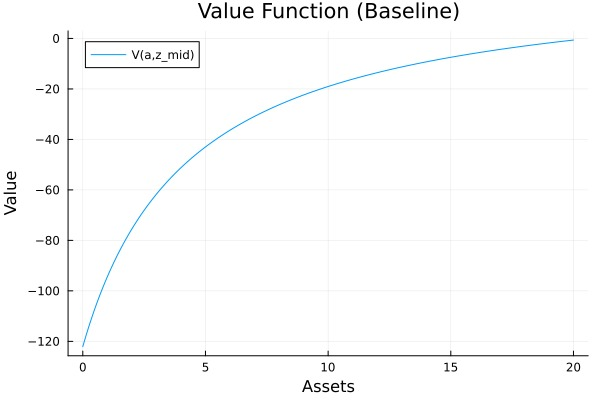
\includegraphics[width=\textwidth]{C:/Users/Shokoufeh/OneDrive/third_semester/QE/QE_problem_set/Quantitative_Economics/project/value_function_baseline.jpg}
    \caption{value function baseline}
\end{minipage}\hfill
\begin{minipage}{0.45\textwidth}
    \centering
    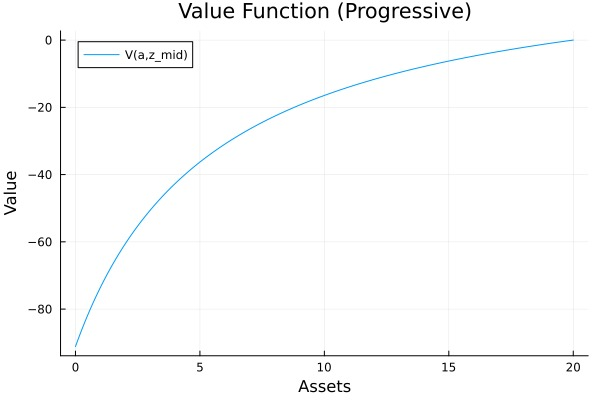
\includegraphics[width=\textwidth]{C:/Users/Shokoufeh/OneDrive/third_semester/QE/QE_problem_set/Quantitative_Economics/project/value_function_progressive.jpg}
    \caption{value function progressive}
\end{minipage}
\end{center}
\end{figure}
\FloatBarrier
\item \textbf{Policy Functions}: Consumption and savings decisions.\\
\begin{figure}[htbp]
\begin{center}
\begin{minipage}{0.45\textwidth}
    \centering
    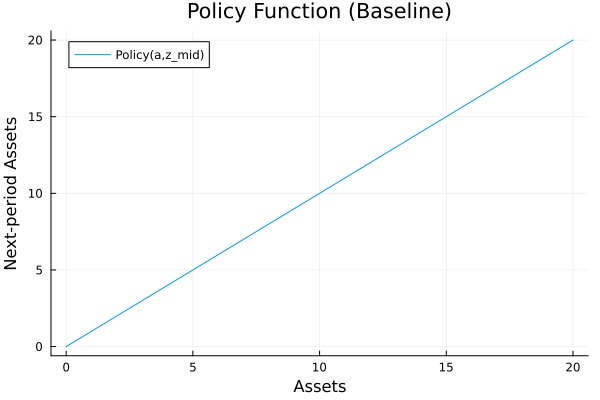
\includegraphics[width=\textwidth]{C:/Users/Shokoufeh/OneDrive/third_semester/QE/QE_problem_set/Quantitative_Economics/project/Policy function baseline.jpg}
    \caption{Policy function baseline}
\end{minipage}\hfill
\begin{minipage}{0.45\textwidth}
    \centering
    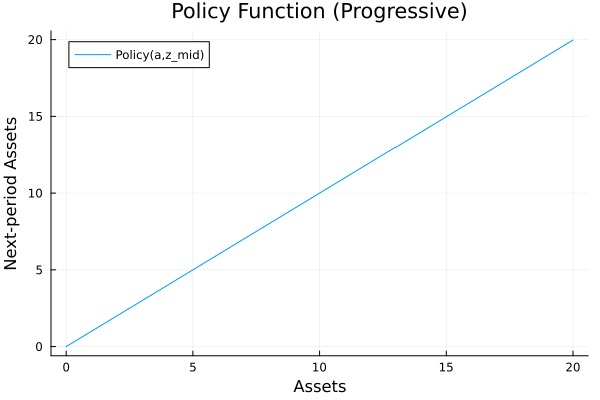
\includegraphics[width=\textwidth]{C:/Users/Shokoufeh/OneDrive/third_semester/QE/QE_problem_set/Quantitative_Economics/project/Policy function progressive.jpg}
    \caption{Policy function progressive}
\end{minipage}
\end{center}
\end{figure}
\FloatBarrier
\item \textbf{Asset Distribution}: Marginal distributions across regimes.\\
\begin{figure}[htbp]
\begin{center}
\begin{minipage}{0.45\textwidth}
    \centering
    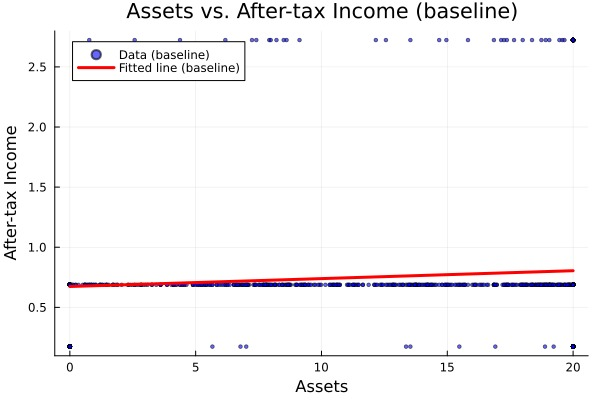
\includegraphics[width=\textwidth]{C:/Users/Shokoufeh/OneDrive/third_semester/QE/QE_problem_set/Quantitative_Economics/project/The marginal distribution of assets baseline.jpg}
    \caption{The marginal distribution of assets baseline}
\end{minipage}\hfill
\begin{minipage}{0.45\textwidth}
    \centering
    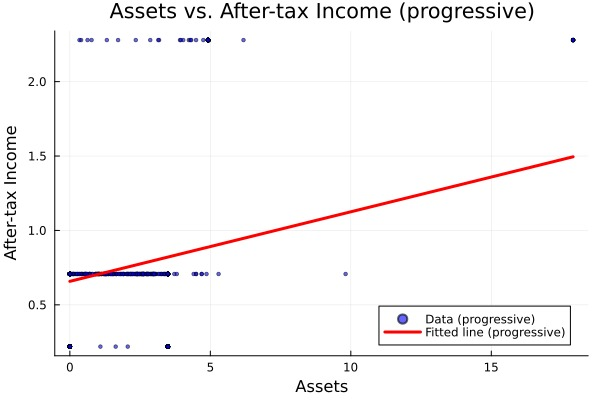
\includegraphics[width=\textwidth]{C:/Users/Shokoufeh/OneDrive/third_semester/QE/QE_problem_set/Quantitative_Economics/project/The marginal distribution of assets progressive.jpg}
    \caption{The marginal distribution of assets progressive}
\end{minipage}
\end{center}
\end{figure}
\FloatBarrier
\item \textbf{Lorenz Curves}: Illustrating inequality changes.\\
\begin{figure}[htbp]
\begin{center}
\begin{minipage}{0.45\textwidth}
    \centering
    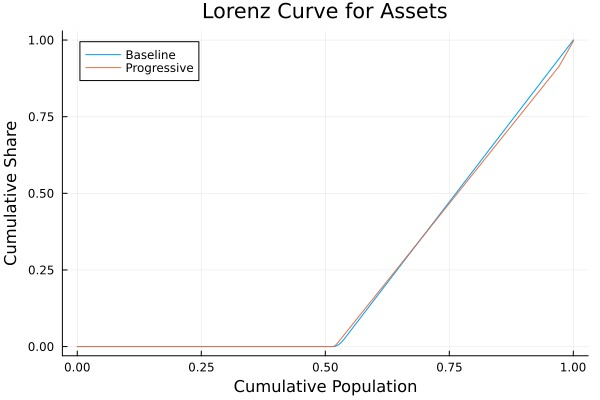
\includegraphics[width=\textwidth]{C:/Users/Shokoufeh/OneDrive/third_semester/QE/QE_problem_set/Quantitative_Economics/project/The Lorenz curves for assets.jpg}
    \caption{The Lorenz curves for assets}
\end{minipage}\hfill
\begin{minipage}{0.45\textwidth}
    \centering
    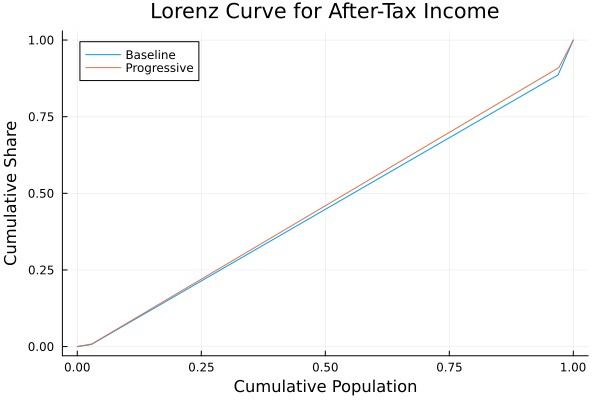
\includegraphics[width=\textwidth]{C:/Users/Shokoufeh/OneDrive/third_semester/QE/QE_problem_set/Quantitative_Economics/project/The Lorenz curves for after-tax labor income.jpg}
    \caption{The Lorenz curves for after-tax labor income}
\end{minipage}
\end{center}
\end{figure}
\FloatBarrier
\end{itemize}

\section{Conclusion}

The results show that increasing tax progressivity effectively reduces income inequality, as seen in the drop in the after-tax Gini coefficient. However, wealth inequality slightly increases, indicating that redistribution primarily affects income rather than long-term asset accumulation. The rise in the capital-to-output ratio and the decline in the interest rate suggest greater capital accumulation, making borrowing cheaper and encouraging investment. While the wage rate increases slightly, the overall tax burden decreases, benefiting lower-income households. These findings highlight the trade-offs between equity and savings incentives in progressive tax policies.

\end{document}
